\chapter{Simulations}
\label{cha:simulations}
This chapter is about the different simulations available with
SimSpark. In particular the soccer simulation is described in detail.\newline





%-SECTION-----------------------------------------------------------
%---------------------- The Soccer Simulation ----------------------
%-------------------------------------------------------------------
\section{The Soccer Simulation}
\label{sec:soccersimulation}
We implemented a simulation for SimSpark where two teams of up to 6
humanoid robots play soccer against each other.
Figure \ref{fig:soccersim} shows a running soccer simulation with $12$ playing
robots of two teams. This seemingly simple setup poses a challenge to agent
implementers on several levels.

In order to act in a meaningful way on the playing field the first
challenge is to localize your agent on the playing field. To support
this the agents perceive their relative position to a set of
landmarks, called \texttt{flags} on the playing field. These flags
mark corner and goal spots of the playing field. Further the relative
location of other players and the ball on the soccer field are perceived.

If an agent knows where it is and where it wants to be in the near
future the next challenge is to walk there. The structure of the
humanoids are sufficiently realistic to make this non trivial. Further
the agent has to recover and get up if fallen over.

Another challenge is kicking the ball. As trivial this sounds to a
human it is far from trivial for a robot to keep its dynamic balance
when kicking and controlling the direction of the ball.

Agents that are able to move and kick the ball need to cooperate and
form a team. Only the effective application of strategic and
cooperative behaviors forms a successful team.

Most rules of the soccer game are judged by an automatic rule set that
enforces the basic soccer rule set. However more involved situations
like detection unfair behavior still require a human referee.\newline

This soccer simulation is also used as the official competition environment for
the 3D Soccer Simulation League at RoboCup\footnote{For more information on
RoboCup, see also \url{http://www.robocup.org/}}
\cite{KAK+97}\cite{KA00}\cite{BMO+05}\cite{MBS+07}. The robots used in the
simulation at the competitions is currently the Nao robot as described in
chapter \ref{cha:robots}.\newline

\begin{figure}[htbp]
  \centering
  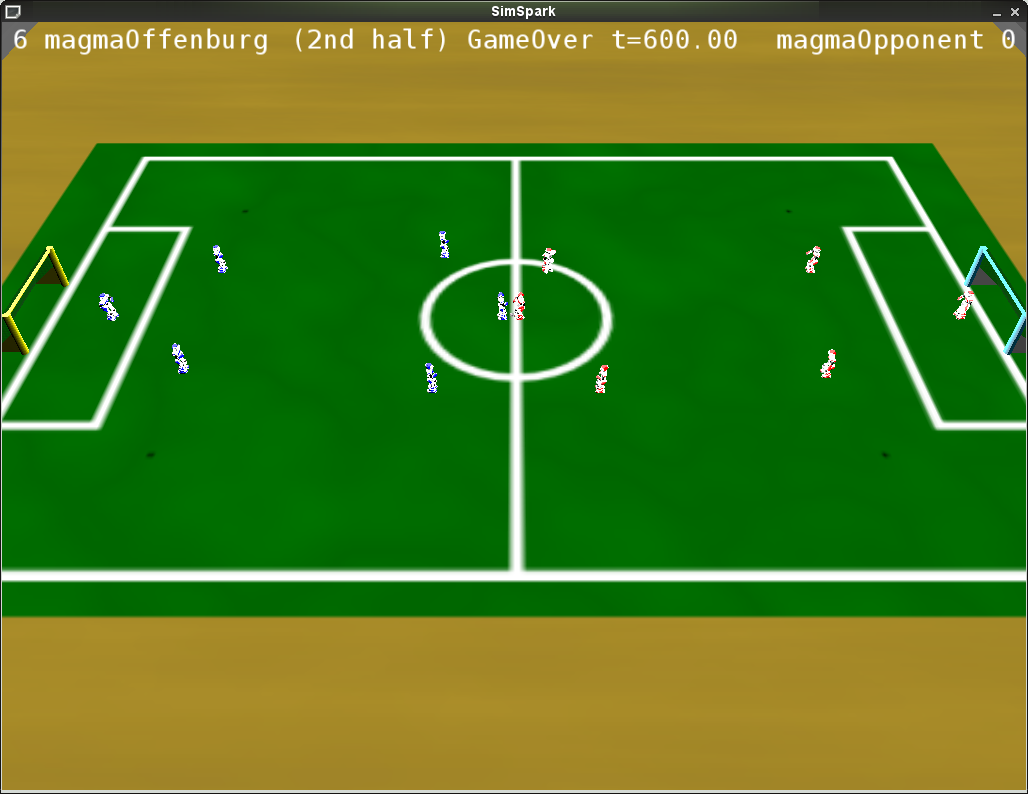
\includegraphics[width=\textwidth]{fig/soccersim}
  \caption{A screen shot of the soccer simulation with 6 vs 6 robots}
  \label{fig:soccersim}
\end{figure}





%-SUB-SECTION-------------------------------------------------------
%-------------- Environment and Objects on the Field ---------------
%-------------------------------------------------------------------
\subsection{Environment and Objects on the Field}
The dimensions of the soccer field are $x=18m$ by $y=12m$. The center spot has a
radius of $1.5$ meters. Each goal is $y=2.1m$ by $x=0.6m$ with a height of
$z=0.8m$. The penalty area to each goal is $y=3.9m$ by $x=1.8m$. The soccer
field is surrounded by a border of $10$ meters in each direction. Space outside
this border area is not reachable by an agent. The soccer ball has a radius of
$0.042$ meter and a mass of $26$ grams. For an up to date list of all values
please refer to (./rcssserver3d/naosoccersim.rb).

At each corner of the soccer field, and at the goal posts, a distinctive
flag is placed. The positions of these flags are fixed and known to
each agent. Agents perceive the relative position of a subset of
these flags and are therefore able to localize themselves on the soccer
field. Agents distinguish flags through their identifier as shown in figure
\ref{fig:pitch}. While the markers for the flags are placed on ground level
($z=0.0m$), the goalpost markers are placed on the top of each goalpost at a
height of $z=0.8m$.

\begin{figure}[htbp]
  \centering
  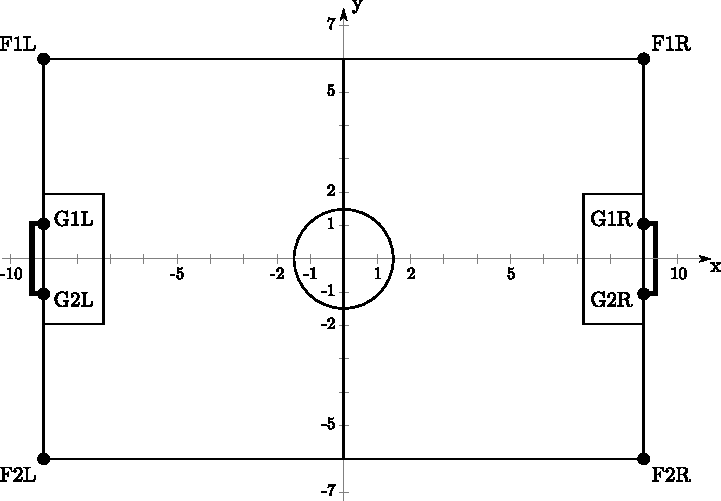
\includegraphics[width=\textwidth]{fig/pitch2}
  \caption{The dimensions of the soccer pitch and the object markers on the
  field as perceived by an agent}
  \label{fig:pitch}
\end{figure}





%-SUB-SECTION-------------------------------------------------------
%-------------- Rules Judged by the Automatic Referee --------------
%-------------------------------------------------------------------
\subsection{Rules Judged by the Automatic Referee}
In order to run a soccer game several rules have to be applied.
The automatic referee automatically limits the time of each game
half. It further keeps track which player was the last one to touch
the ball and checks whether the ball enters the goal penalty areas of
the soccer field, or was kicked into touch. Therefore it is able to detect and
score \texttt{goals}, automatically judge \texttt{ball out} and give \texttt{kick
in}, \texttt{corner kick in} or \texttt{goal kick} to the correct team. The
\texttt{offside} rule is implemented but still experimental.
During a \texttt{free kick}, the opponent team has to keep a minimum distance of
$1.3$ meter, as well as $1.0$ meter in case of a \texttt{goal kick}. 

With SimSpark Version 1.3 several new rules were applied to the automatic
referee, in order to ensure a smooth gameplay. 
The automatic referee tries to avoid mass collisions of robots around the ball,
as well as dead robots lying around on the field, blocking the gameplay.
Furthermore it takes care that no team is blocking the own goal with more than
a certain amount of players. In all cases the robots causing the problem
situation are automatically beamed outside the soccer field. For an up to date
list of all values please refer to (./rcssserver3d/naosoccersim.rb).





%-SUB-SECTION-------------------------------------------------------
%---------------- Rules Judged by the Human Referee ----------------
%-------------------------------------------------------------------
\subsection{Rules Judged by the Human Referee}

The human referee acts through a connected monitor. It is responsible
to give the \texttt{kick off} command to start each game half. The
automatic referee currently does not resolve situations where the game
got stuck if for example several player block each other and no one is
able to reach the ball. Further it does not detect fouls like the use
of hands or otherwise behavior on the soccer field.

In these cases the human referee can \texttt{drop ball} the ball,
i.e. put it on a random location on the playing field to unstuck the
game. He is further able to command a \texttt{free kick} where one
player is able to shoot from a short distance to the goal.

%\subsection{Setup Script}


%%% Local Variables: 
%%% mode: latex
%%% TeX-master: "user-manual"
%%% End: 
